
\chapter{فهرست ‌اولویت‌بندی‌شده ریسک‌ها}

\section{فهرست ریسک‌ها}
\subsection{ریسک‌های مربوط به محدوده و نیازمندی‌ها}

\subsubsection{روشن نبودن محدوده پروژه}
\paragraph{توضیح}
تعریف دقیق و واضحی از نیازمندی‌های سیستم و جزییات سناریوهایی که در سازمان رخ می‌دهد ارائه نشده است.
\paragraph{راه‌حل}
پس از مکاتبه با دستیار آموزشی، تا حدی شفاف‌سازی صورت گرفت.
%%%%%%%%%%%%%%%%%%%%%%%%%%%%%%%%%%%%%%%%%%%%%%%%%%%
\subsubsection{درک نادرست نیازمندی‌ها توسط تیم ایجاد}
\paragraph{توضیح}
درک نادرست نیازمندی‌ها باعث می‌شود از اولین فاز تحلیل‌ها نادرست باشد و در انتها منجر به طراحی و پیاده‌سازی اشتباه شود.
\paragraph{راه‌حل}
تعامل بیشتر با دستیاران آموزشی  در طول انجام پروژه بهترین روش برای مقابله با این ریسک است.

%%%%%%%%%%%%%%%%%%%%%%%%%%%%%%%%%%%%%%%%%%%%%%%%%%
\subsubsection{چندپهلو بودن نیازمندی‌ها}
\paragraph{توضیح}
چندپهلو بودن نیازمندی‌ها می‌تواند باعث هدر رفتن زمان قابل توجهی از فاز تحلیل برای ابهام‌زدایی از نیازمندی‌ها و در نهایت منجر به پیاده‌سازی نیازمندی‌های نادرست شود.
\paragraph{راه‌حل}
تعامل بیشتر با دستیاران آموزشی برای دریافت بازخورد، بهترین روش برای مقابله با این ریسک است.
%%%%%%%%%%%%%%%%%%%%%%%%%%%%%%%%%%%%%%%%%%%%%%%%%%
\subsubsection{بزرگ شدن بیش از حد پروژه}
\paragraph{توضیح}
در صورتی که تیم بیش از حد به جزییات بپردازد، ممکن است محدوده‌ی پروژه از حد مطلوب خیلی بزرگتر شود.
\paragraph{راه‌حل}
مرور دوره ای مستندات نیازمندی که هنگام تعامل با کاربر بدست آمده است، می تواند راه حلی جهت مقابله با این ریسک باشد.
%%%%%%%%%%%%%%%%%%%%%%%%%%%%%%%%%%%%%%%%%%%%%%%%%%
\subsection{ریسک‌های مربوط به زمان‌بندی}
\subsubsection{تخمین‌های زمانی نادرست برای انجام تسک‌ها}
\paragraph{توضیح}
بر اثر بی‌تجربگی اعضا، عدم تسلط بر تکنولوژی‌های مورد استفاده و اتفاق‌های پیش‌بینی نشده، ممکن است تخمین‌های زمانی تفاوت زیادی با زمان صرف شده واقعی داشته باشند که منجر به عدم تحویل به موقع پروژه خواهد شد.
\paragraph{راه‌حل}
استفاده از تجارب دیگران و بررسی برنامه زمانبندی پروژه های مشابه، بهترین روش برای مقابله با این ریسک است.
%%%%%%%%%%%%%%%%%%%%%%%%%%%%%%%%%%%%%%%%%%%%%%%%%%
\subsubsection{اعلام دیرهنگام بسترهای مجاز برای انجام پروژه}
\paragraph{توضیح}
این مورد ممکن است که به تاخیر در یادگیری یک بستر جدید منجر شود که در نهایت به تاخیر در تحویل پروژه بیانجامد.
\paragraph{راه‌حل}
پیگیری زودهنگام اعضای گروه در مورد تکنولوژی هایی که به نظر ایشان مناسب و مجاز است، راه حل پیشگیری این ریسک است.
%%%%%%%%%%%%%%%%%%%%%%%%%%%%%%%%%%%%%%%%%%%%%%%%%%
\subsection{ریسک‌های مربوط به مدیریت تغییرات}
\subsubsection{ناسازگاری بین محصولات}
\paragraph{توضیح}
در صورتی که میان محصولات تولید شده در فازهای مختلف سازگاری وجود نداشته باشد، ممکن است کیفیت محصولات هر فاز نسبت به فاز قبلی کاهش پیدا کند. همچنین، فاصله گرفتن از یافته‌های فازهای قبل، می‌تواند منجر به ارضای نادرست نیازمندی‌ها شود.
\paragraph{راه‌حل}
برای جلوگیری از بروز این ریسک دو راه حل متصور است:
\begin{enumerate}
	\item استفاده از تکنولوژی های مناسب که کنترل سازگاری را به صورت خودکار پشتیبانی می کنند.
	\item کنترل سازگاری محصولات در پایان هر فاز با فاز قبل توسط اعضای تیم.
\end{enumerate}
\subsection{ریسک‌های مربوط به ارتباطات}

\subsubsection{کمرنگ شدن ارتباط دستیاران با تیم}
\paragraph{توضیح}
فعالیت دستیاران درس در طول ترم کمرنگ شود و بازخوردها به موقع ارائه نشوند.
\paragraph{راه‌حل}
در ابتدای هر تکرار، سوالات بحرانی از قبیل سررسید
\LTRfootnote{Deadline}
و ابهامات موجود در مورد خواسته ها از دستیاران محترم پرسیده شود.
%%%%%%%%%%%%%%%%%%%%%%%%%%%%%%%%%%%%%%%%%%%%%%%%%%
\subsubsection{مورد قبول واقع نشدن محصول نهایی}
\paragraph{توضیح}
در صورتی که محصول نهایی در آزمون پذیرش رد شود، هر چقدر هم که از استانداردهای کیفی تبعیت کرده باشد، پروژه شکست خورده اعلام خواهد شد.
\paragraph{راه‌حل}
با تحلیل دقیق، تعامل بیشتر با مشتری و اعمال بازخوردهای هر فاز، می‌توان ریسک مورد قبول واقع نشدن محصول نهایی را کاهش داد.
%%%%%%%%%%%%%%%%%%%%%%%%%%%%%%%%%%%%%%%%%%%%%%%%%%

\subsection{ریسک‌های مربوط به نیروی انسانی}
%%%%%%%%%%%%%%%%%%%%%%%%%%%%%%%%%%%%%%%%%%%%%%%%%%
\subsubsection{خروج عضوی از تیم پیش از پایان یافتن پروژه}
\paragraph{توضیح}
یکی از اعضای تیم، پیش از پایان یافتن پروژه ممکن است جهت تحصیل در خارج از کشور مهاجرت کند و از تیم خارج شود.
\paragraph{راه‌حل}
سه راه‌حل برای این ریسک قابل تصور است که به اقتضای موقعیت، یکی باید انتخاب شود:
\begin{enumerate}
	\item انجام تسک‌ها به صورت فشرده‌ای باشد تا پیش از مهاجرت عضو، پروژه پایان یافته باشد.
	\item در حین انجام پروژه، بقیه اعضای تیم در جریان جزییات تسک‌هایی که آن فرد انجام می‌دهد قرار گیرند تا بتوانند در صورت لزوم ادامه‌ی تسک‌های وی را انجام دهند.
	\item امکان برقراری ارتباط از راه دور با عضو خارج شده میسر باشد تا همکاری بدین صورت انجام شود.
\end{enumerate}
%%%%%%%%%%%%%%%%%%%%%%%%%%%%%%%%%%%%%%%%%%%%%%%%%%
\subsubsection{اتفاقات غیرمترقبه}
\paragraph{توضیح}
برای نمونه، امتحان‌های درسی ممکن است منجر به در دسترس نبودن یک یا چند عضو در یک بازه زمانی بحرانی شود.
\paragraph{راه‌حل}
در هنگام تخمین‌های زمانی، باید این موارد تا حد امکان در نظر گرفته شوند.
%%%%%%%%%%%%%%%%%%%%%%%%%%%%%%%%%%%%%%%%%%%%%%%%%%
\subsubsection{درگیر شدن اعضای تیم در پروژه‌های دیگر}
\paragraph{توضیح}
پروژه‌های درس‌های دیگر ممکن است باعث شود که برنامه‌ریزی‌ها با مشکل مواجه شوند که خود می‌تواند منجر به کاهش کیفیت محصولات ترخیص شود.
\paragraph{راه‌حل}
برنامه ریزی و اولویت بندی مناسب پروژه ها، عواقب این ریسک را کاهش می دهد.
%%%%%%%%%%%%%%%%%%%%%%%%%%%%%%%%%%%%%%%%%%%%%%%%%%

\subsection{ریسک‌های تکنیکی}

\subsubsection{بروز مشکلات سخت‌افزاری و نرم‌افزاری}
\paragraph{توضیح}
برای نمونه خراب شدن کامپیوتر/لپ‌تاپ یکی از اعضای تیم، بروز ایراد طولانی مدت در اتصال اینترنت یا بروز اشکال طولانی مدت برای Trello یا Telegram یا Github. در صورتی که هر یک از این اتفاقات رخ دهد، زمان‌بندی‌ها با مشکل مواجه می‌شود. در مورد بروز مشکلات در سه مورد آخر، ارتباط  از راه دور نیز برای اعضای تیم دشوار می‌گردد.
\paragraph{راه‌حل}
لازم است سعی شود همواره یک رونوشت از آخرین محصولات به صورت برون‌خط\LTRfootnote{Offline} موجود باشد تا در صورت آسیب کامپیوتر اعضا یا عدم امکان برقراری ارتباط با سایت Github، کماکان بتوان روی کدها کار کرد. \\
از آن‌جاییکه که نگهداری مستندات و تقسیم وظایف از طریق Trello انجام می‌گردد، در صورتی که تقسیم کار و مستندات را به صورت برون‌خط داشته باشیم، در صورت بروز ایراد در Trello مشکلی جدی برای تیم رخ نخواهد داد. \\
در صورتی که Telegram با مشکلات قطعی مواجه شود، می‌توان از خدمات جایگزین، مانند ایمیل استفاده کرد.
%%%%%%%%%%%%%%%%%%%%%%%%%%%%%%%%%%%%%%%%%%%%%%%%%%
\subsubsection{نیاز به یادگیری مهارت‌های جدید}
\paragraph{توضیح}
ممکن است لازم شود اعضای تیم موارد جدیدی را یاد بگیرند که باعث نادقیق بودن تخمین‌های زمانی شود.
\paragraph{راه‌حل}
یادگیری مهارت های جدید از طریق منابع مناسب نظیر ویدئوهای موجود و استفاده از تجارب افراد متخصص در ان زمینه که باعث تسریع یادگیری استفاده از آن تکنولوژی می شود.
%%%%%%%%%%%%%%%%%%%%%%%%%%%%%%%%%%%%%%%%%%%%%%%%%%
\subsubsection{نامناسب بودن ابزارهای CASE مورد استفاده}
\paragraph{توضیح}
ممکن است ابزارهای CASE مورد استفاده، بعضی از نمودارهایی را که لازم است تولید شوند پشتیبانی نکند. در نتیجه هماهنگ کردن نمودارهای مختلف با یکدیگر ممکن است مشکل‌ساز شود.\\
همچنین، ممکن است اعضای تیم ایجاد شناخت دقیقی از ابزار CASE مورد استفاده نداشته باشند و انتظاری داشته باشند که با این ابزار قابل رفع نباشد. \\
ریسک دیگری که در رابطه با ابزارهای CASE در فاز تحلیل تفصیلی، به علت زیاد بودن تعداد و انواع نمودارها مطرح می‌شود، عدم امکان کار گروهی روی پرونده‌هایی است که این ابزارها تولید می‌کنند که باعث بروز عدم یکپارچگی می‌شود. ({\color{red} بهنگام‌سازی شد.})

\paragraph{راه‌حل}
تشویق اعضای تیم به مطالعه‌ی دقیق مستندات و 
راهنماهای ابزارهای مختلف CASE پیش از انتخاب و استفاده تا حد خوبی این ریسک را کاهش می‌دهد. \\
برای مقابله با ریسک مربوط به عدم یکپارچگی، لازم است هماهنگی بین اعضای گروه صورت گیرد و در هر زمان حداکثر یک نفر روی یک پرونده کار کند.
%%%%%%%%%%%%%%%%%%%%%%%%%%%%%%%%%%%%%%%%%%%%%%%%%%
\subsubsection{نامناسب بودن ابزار مدیریت پروژه}
\paragraph{توضیح}
نرم‌افزار 
\lr{MS Project}
که از آن برای رسم نمودار گانت
\LTRfootnote{Gantt}
و پرت
\LTRfootnote{Pert}
استفاده می‌کنیم، از تقویم هجری شمسی پشتیبانی نمی‌کند و استفاده از تاریخ میلادی برای زمان‌بندی کمی دشوار است. همچنین در مستند پروژه لازم است تاریخ‌ها به صورت شمسی ذکر گردند.
\paragraph{راه‌حل}
یک راه‌حل این است که ماکرویی برای تبدیل تاریخ میلادی به شمسی ایجاد شود. یک راه‌حل  میانی هم وجود دارد و این است که زمان‌بندی‌ها را در قالب تاریخ میلادی انجام دهیم و پیش از انتقال زمان‌بندی بهنگام‌شده به مستند پروژه، تاریخ‌ها را به صورت دستی به هجری شمسی تبدیل کنیم.
%%%%%%%%%%%%%%%%%%%%%%%%%%%%%%%%%%%%%%%%%%%%%%%%%%
\subsubsection{دشواری‌های مربوط به ارتباط با پایگاه‌داده}
\paragraph{توضیح}
ممکن است در هنگام پیاده‌سازی، برای برقراری ارتباط با پایگاه داده مشکلاتی از لحاظ فنی رخ بدهد که به علت عدم تحربه‌ی کافی اعضا در این زمینه، محتمل است. در صورت وقوع، تخمین‌های زمانی با مشکل مواجه خواهد شد.
\paragraph{راه‌حل}
تهیه Executable Architectural Baseline باعث اطمینان حاصل کردن از توانایی اتصال پایگاه داده و توانایی ارتباط برقرار کردن با آن به کمک wrapper های موجود (JPA) شد.
%%%%%%%%%%%%%%%%%%%%%%%%%%%%%%%%%%%%%%%%%%%%%%%%%%

\section{اولویت‌بندی ریسک‌ها}
برای اولویت‌بندی ریسک‌های موجود، باید به احتمال وقوع و شدت عواقب هر یک در صورت وقوع توجه کرد. از این رو نمودار نقطه‌ای ریسک‌ها را برحسب این دو معیار رسم می‌کنیم.\\

\begin{figure}[H]
	\centering
	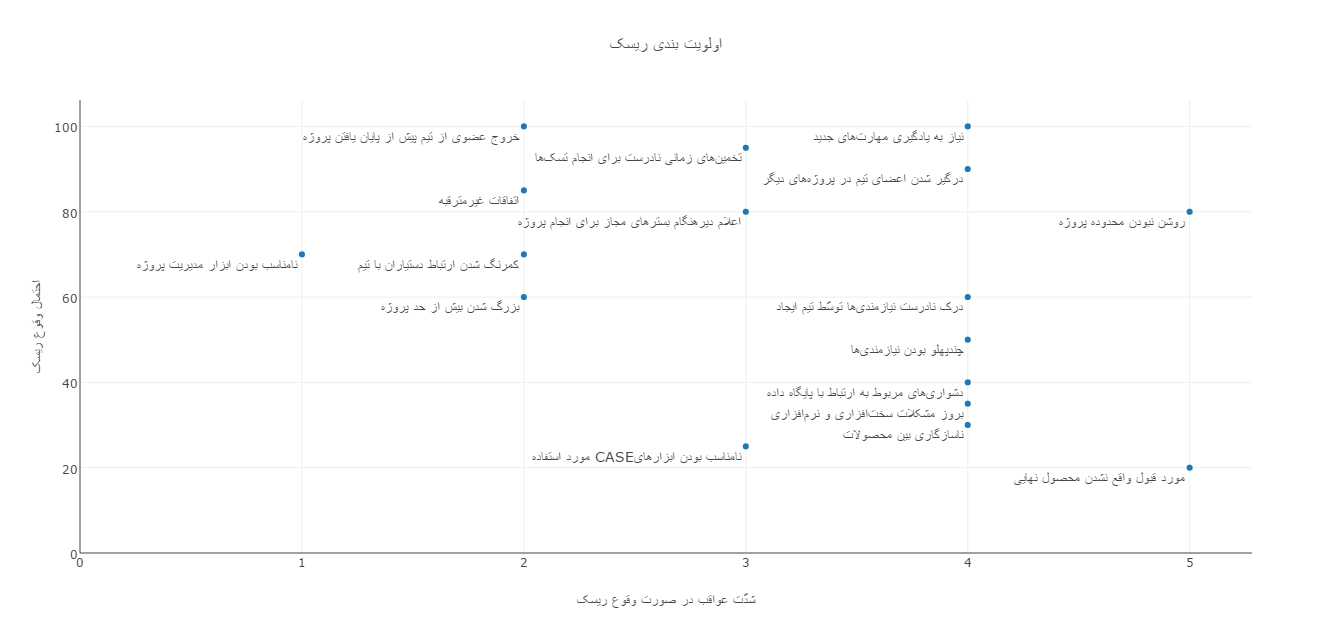
\includegraphics[scale=0.3]{img/risk_prioritization}
%	\caption{زیرسیستم گزارش‌گیری}
\end{figure}

با توجه به معیارهای هر محور، می‌توان گفت هر چه ریسک در نمودار به سمت گوشه‌ی بالا راست متمایل باشد، تهدید بزرگتری برای موفقیت پروژه محسوب می‌شود. از این رو اولویت ریسک‌ها به ترتیب زیر است:\\
\begin{enumerate}
	\item روشن نبودن محدوده‌ی پروژه
	\item نیاز به یادگیری مهارت‌های جدید
	\item درگیر شدن اعضای تیم در پروژه‌های دیگر
	\item درک نادرست نیازمندی‌ها توسط تیم ایجاد
	\item تخمین‌های زمانی نادرست برای انجام تسک‌ها
	\item اعلام دیرهنگام بسترهای مجاز برای انجام پروژه
	\item چندپهلو بودن نیازمندی‌ها
	\item مورد قبول واقع نشدن محصول نهایی
	\item خروج عضوی از تیم پیش از پایان یافتن پروژه
	\item اتفاقات غیرمترقبه
	\item دشواری‌های مربوط به ارتباط با پایگاه‌داده
	\item بروز مشکلات سخت‌افزاری و نرم‌افزاری
	\item ناسازگاری بین محصولات
	\item کم‌رنگ شدن ارتباط دستیاران با تیم
	\item بزرگ شدن بیش از حد پروژه
	\item نامناسب بودن ابزارهای CASE مورد استفاده
	\item نامناسب بودن ابزار مدیریت پروژه
\end{enumerate}
